\chapter{Software Design}

\section{General Architecture}

My application will be written in Swift and SwiftUI. The file architecture diagram below serves as the foundational blueprint for my application. This visual representation offers a high-level overview of how data and functionalities are organized within the application. It outlines the structure of the app, showcasing the relationships between various components, data storage, and user interfaces. The teal files represent UI-level views, whereas the grey files represent classes that are at a lower level.

\begin{figure}[H]
    \centering
    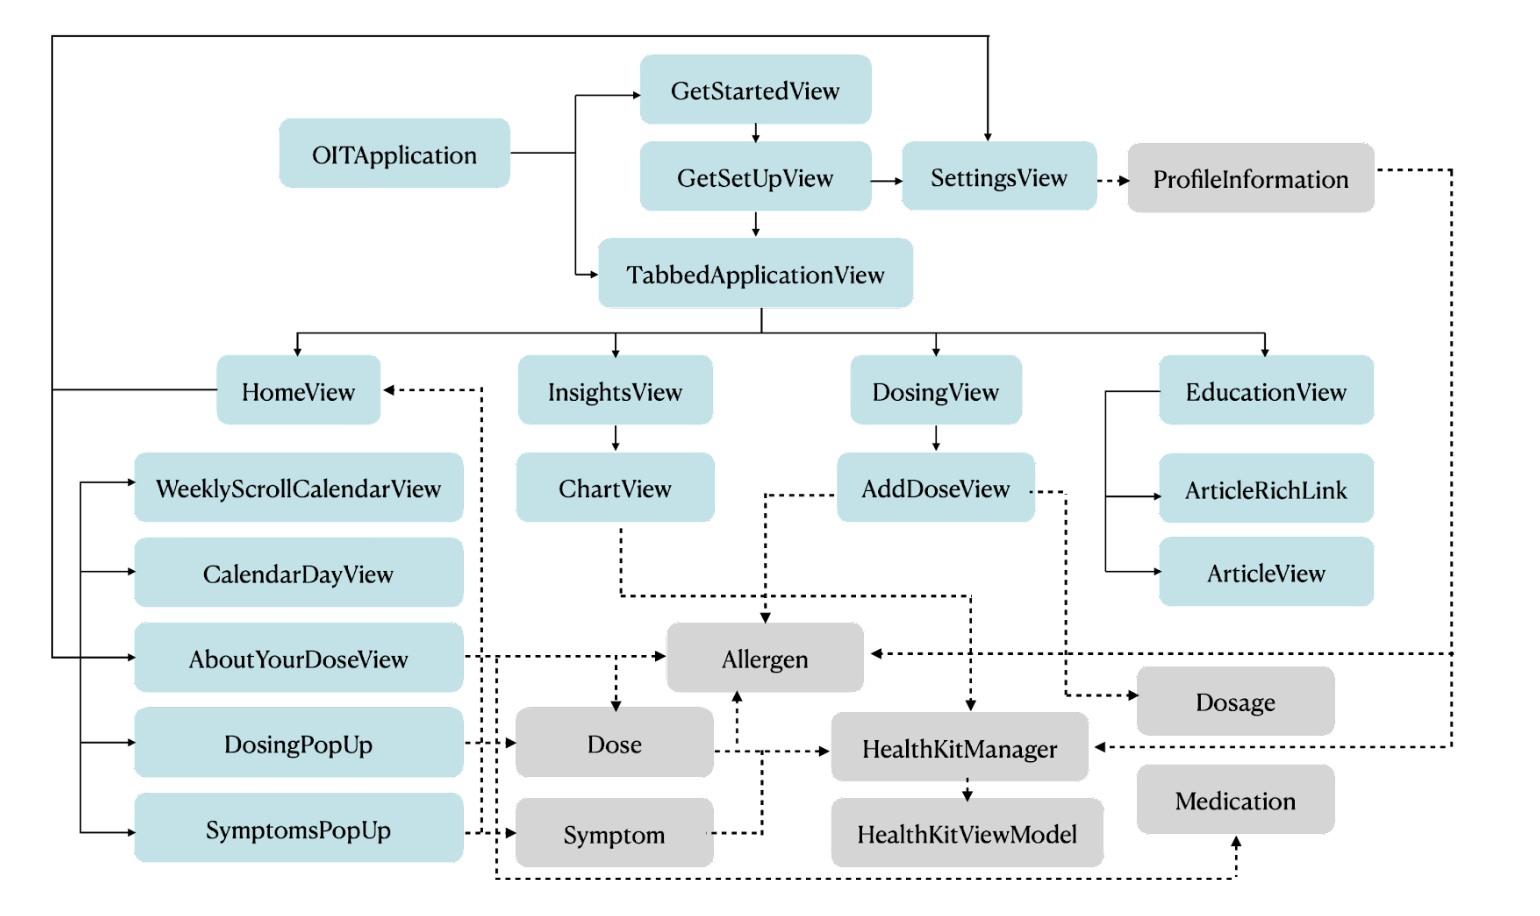
\includegraphics[width=1\linewidth]{thesis/chapters/images/overallFileArchitecture.png}
    \caption{Overall File Architecture}
    \label{fig:overall-file-architecture}
\end{figure}

\section{APIs}

Leveraging a combination of powerful APIs, my application aims to provide an enhanced and user-centric healthcare experience. I plan to utilize HealthKit, an integral component of the iOS ecosystem, which acts as a central repository for health and fitness data. With the user's explicit consent, my application will seamlessly integrate with HealthKit, facilitating the access and sharing of vital health information from the user's iPhone and Apple Watch \cite{HealthKit}. This integration will not only enable the application to provide personalized insights but also enhance the accuracy and reliability of the data we collect.

In addition, CareKit stands as another essential pillar in my app's framework. CareKit empowers users to take control of their health, enabling us to offer functionalities that support trend analysis, goal setting, and incentives. With CareKit 2.0's availability for iOS 13 and iPadOS 13 and above, my app will be able to provide a comprehensive health management experience, fostering a proactive approach to Oral Immunotherapy \cite{CareKit}.

To transform data into informative visualizations and offer a visually appealing user interface, I plan to implement the Swift Charts framework. Swift Charts offers a concise SwiftUI-based solution for creating a wide array of customizable charts \cite{SwiftCharts}. This powerful tool provides a range of essential building blocks, such as marks, scales, axes, and legends, which I can creatively combine to develop interactive and data-driven charts. These visualizations will not only enhance the user's understanding of their OIT journey but also make the app more engaging and informative.

Lastly, Swift Data will play a pivotal role in ensuring data persistence and accessibility across app launches. This framework simplifies the management of custom data types, making it easier to store and retrieve information efficiently \cite{SwiftData}. By integrating Swift Data with SwiftUI, I can seamlessly fetch and display key data, creating a seamless and reliable user experience. Whether it's preserving user progress or maintaining essential healthcare records, Swift Data will be instrumental in maintaining data integrity and availability.

By harnessing the capabilities of HealthKit, CareKit, Swift Charts, and Swift Data, I aim to deliver a comprehensive, informative, and user-friendly platform for individuals undergoing oral immunotherapy, transforming the way they manage their health and improve their overall well-being.

\section{Class diagrams}

The Class Diagrams below serve as a blueprint for the software development of the application. By visually representing classes and their attributes, this section delves into the heart of the application's design. Following UML standards, each diagram shows the private and public variables and methods for the class.

\begin{table}[ht]
\centering
\caption{Class Diagram: OITApplication}

\hspace{1em}
\renewcommand{\arraystretch}{1.7}

\begin{tabular}{|l|}
\hline
\textbf{OITApplication} \\
\hline
– hasAppBeenOpenedBefore: Bool \\
\hline
\end{tabular}
\end{table}

\begin{table}[H]
\centering
\caption{Class Diagram: TabbedApplicationView}

\hspace{1em}
\renewcommand{\arraystretch}{1.7}

\begin{tabular}{|l|}
\hline
\textbf{TabbedApplicationView} \\
\hline
– homeViewTab: NavigationView \\
– insightsViewTab: NavigationView \\
– dosingViewTab: NavigationView \\
– educationViewTab: NavigationView \\
\hline
\end{tabular}
\end{table}

\begin{table}[H]
\centering
\caption{Class Diagram: GetStartedView}

\hspace{1em}
\renewcommand{\arraystretch}{1.7}

\begin{tabular}{|l|}
\hline
\textbf{GetStartedView} \\
\hline
– getStartedButton: Button \\
– appTitle: Text \\
– backgroundColor: Color \\
\hline
\end{tabular}
\end{table}

\begin{table}[H]
\centering
\caption{Class Diagram: GetSetUpView}

\hspace{1em}
\renewcommand{\arraystretch}{1.7}

\begin{tabular}{|l|}
\hline
\textbf{GetSetUpView} \\
\hline
– title: String \\
+ personalInformation: ProfileInformation \\
– settingsView: SettingsView \\
– getStartedButton: Button \\
\hline
\end{tabular}
\end{table}

\begin{table}[H]
\centering
\caption{Class Diagram: ProfileInformation}

\hspace{1em}
\renewcommand{\arraystretch}{1.7}

\begin{tabular}{|l|}
\hline
\textbf{ProfileInformation} \\
\hline
+ name: String \\
+ birthdate: Date \\
+ allergens: [Allergen] \\
+ shareDataWithAppleHealth: Bool \\
+ protectDataWithFaceID: Bool \\
\hline
\end{tabular}
\end{table}

\begin{table}[H]
\centering
\caption{Class Diagram: Allergen}

\hspace{1em}
\renewcommand{\arraystretch}{1.7}

\begin{tabular}{|l|}
\hline
\textbf{Allergen} \\
\hline
– AllergenType: enumeration(String) \\
+ allergen: AllergenType \\
\hline
\end{tabular}
\end{table}

\begin{table}[H]
\centering
\caption{Class Diagram: Symptom}

\hspace{1em}
\renewcommand{\arraystretch}{1.7}

\begin{tabular}{|l|}
\hline
\textbf{Symptom} \\
\hline
– SymptomType: enumeration(HKCategoryType) \\
+ symptom: HKCategoryType \\
\hdashline
+ getSymptomString( ): String \\
\hline
\end{tabular}
\end{table}

\begin{table}[ht]
\centering
\caption{Class Diagram: Medication}

\hspace{1em}
\renewcommand{\arraystretch}{1.7}

\begin{tabular}{|l|}
\hline
\textbf{Medication} \\
\hline
– MedicationType: enumeration(HKClinicalTypeIdentifier) \\
+ medication: HKClinicalTypeIdentifier \\
\hdashline
+ getMedicationString( ): String \\
\hline
\end{tabular}
\end{table}

\begin{table}[H]
\centering
\caption{Class Diagram: SymptomsPopUp}

\hspace{1em}
\renewcommand{\arraystretch}{1.7}

\begin{tabular}{|l|}
\hline
\textbf{SymptomsPopUp} \\
\hline
+ symptomsSelected: [Symptom] \\
- symptomsButtons: [Button] \\
\hdashline
– changeButtonAppearance( ): Void \\
\hline
\end{tabular}
\end{table}

\begin{table}[H]
\centering
\caption{Class Diagram: HomeView}

\hspace{1em}
\renewcommand{\arraystretch}{1.7}

\begin{tabular}{|l|}
\hline
\textbf{HomeView} \\
\hline
– todayDate: Date \\
+ selectedDate: Date \\
– weekView: Bool \\
– logSymptoms: Bool \\
– logDose: Bool \\
– profileButton: Button \\
– calendarButton: Button \\
– weeklyScrollCalendarView: WeeklyScrollCalendarView \\
– logDoseButton: Button \\
– logSymptomsButton: Button \\
– aboutYourDoseView: AboutYourDoseView \\
– dose: Dose \\
– symptoms: Symptoms \\
\hline
\end{tabular}
\end{table}

\begin{table}[H]
\centering
\caption{Class Diagram: WeeklyScrollCalendarView}

\hspace{1em}
\renewcommand{\arraystretch}{1.7}

\begin{tabular}{|l|}
\hline
\textbf{WeeklyScrollCalendarView} \\
\hline
– scrollView: ScrollView \\
– dayCircle: CalendarDayView \\
\hdashline
+ startOfWeek( ): Date \\
+ monthHeader( ): String \\
\hline
\end{tabular}
\end{table}

\begin{table}[ht]
\centering
\caption{Class Diagram: CalendarDayView}

\hspace{1em}
\renewcommand{\arraystretch}{1.7}

\begin{tabular}{|l|}
\hline
\textbf{CalendarDayView} \\
\hline
– date: Date \\
– isSelected: Bool \\
– dayText: Text \\
– dateText: Text \\
\hdashline
+ getDayText( ): String \\
+ getDateText( ): String \\
\hline
\end{tabular}
\end{table}

\begin{table}[H]
\centering
\caption{Class Diagram: AboutYourDoseView}

\hspace{1em}
\renewcommand{\arraystretch}{1.7}

\begin{tabular}{|l|}
\hline
\textbf{AboutYourDoseView} \\
\hline
– titleText: Text \\
– allergenText: Text \\
– timeOfDose: Date \\
– dose: Dose \\
– doseIcon: Image \\
\hline
\end{tabular}
\end{table}

\begin{table}[ht]
\centering
\caption{Class Diagram: Dose}

\hspace{1em}
\renewcommand{\arraystretch}{1.7}

\begin{tabular}{|l|}
\hline
\textbf{Dose} \\
\hline
+ name: String \\
+ allergens: [Allergen] \\
+ dosages: [[Allergen, float]] \\
+ dateOfDose: Date \\
+ timeOfDose: Date \\
+ preDoseMedications: [Medication] \\
+ notes: String \\
\hline
\end{tabular}
\end{table}

\begin{table}[H]
\centering
\caption{Class Diagram: DosingPopUp}

\hspace{1em}
\renewcommand{\arraystretch}{1.7}

\begin{tabular}{|l|}
\hline
\textbf{DosingPopUp} \\
\hline
+ dose: Dose \\
– allergenButtons: [Button] \\
– saveDoseButton: Button \\
\hdashline
– saveDose( ): Void \\
\hline
\end{tabular}
\end{table}

\begin{table}[H]
\centering
\caption{Class Diagram: SettingsView}

\hspace{1em}
\renewcommand{\arraystretch}{1.7}

\begin{tabular}{|l|}
\hline
\textbf{SettingsView} \\
\hline
+ personalInformation: ProfileInformation \\
- nameTextField: TextField \\
- birthdateDatePicker: DatePicker \\
- addAllergenButton: Button \\
- shareDataWithAppleHealth: Toggle \\
- enableFaceID: Toggle \\
\hline
\end{tabular}
\end{table}

\begin{table}[H]
\centering
\caption{Class Diagram: HealthKitManager}

\hspace{1em}
\renewcommand{\arraystretch}{1.7}

\begin{tabular}{|l|}
\hline
\textbf{HealthKitManager} \\
\hline
+ symptoms: [HKCategoryType] \\
– dataToRead: [HKCategoryType] \\
– dataToWrite: [HategoryType] \\
\hdashline
+ setUpHealthRequest() \\
\hline
\end{tabular}
\end{table}

\begin{table}[H]
\centering
\caption{Class Diagram: HealthKitViewModel}

\hspace{1em}
\renewcommand{\arraystretch}{1.7}

\begin{tabular}{|l|}
\hline
\textbf{HealthKitViewModel} \\
\hline
+ healthStore: HKHealthStore \\
+ healthKitManager: HKManager \\
+ isAuthorized: Bool \\
\hdashline
+ healthRequest() \\
+ changeAuthorizationStatus() \\
\hline
\end{tabular}
\end{table}

\begin{table}[H]
\centering
\caption{Class Diagram: InsightsView}

\hspace{1em}
\renewcommand{\arraystretch}{1.7}

\begin{tabular}{|l|}
\hline
\textbf{InsightsView} \\
\hline
– title: Text \\
- charts: [ChartView] \\
\hline
\end{tabular}
\end{table}

\begin{table}[H]
\centering
\caption{Class Diagram: ChartView}

\hspace{1em}
\renewcommand{\arraystretch}{1.7}

\begin{tabular}{|l|}
\hline
\textbf{ChartView} \\
\hline
– chartType: Chart \\
– chartData: [AnyObject] \\
\hline
\end{tabular}
\end{table}

\begin{table}[H]
\centering
\caption{Class Diagram: DosingView}

\hspace{1em}
\renewcommand{\arraystretch}{1.7}

\begin{tabular}{|l|}
\hline
\textbf{DosingView} \\
\hline
- title: Text \\
– addNewDoseButton: Button \\
+ allergensAndDoses: [Allergen, [Dosage]] \\
- tableView: TableView \\
\hline
\end{tabular}
\end{table}

\begin{table}[H]
\centering
\caption{Class Diagram: AddDoseView}

\hspace{1em}
\renewcommand{\arraystretch}{1.7}

\begin{tabular}{|l|}
\hline
\textbf{AddDoseView} \\
\hline
– allergen: Picker \\
– nameOfDose: TextField \\
– dosage: TextField \\
– notes: TextField \\
– saveDosageButton: Button \\
+ savedDosage: Dosage \\
\hline
\end{tabular}
\end{table}

\begin{table}[H]
\centering
\caption{Class Diagram: Dosage}

\hspace{1em}
\renewcommand{\arraystretch}{1.7}

\begin{tabular}{|l|}
\hline
\textbf{Dosage} \\
\hline
+ allergen: Allergen \\
+ nameOfDose: String \\
+ dosage: Int \\
+ notes: String \\
\hline
\end{tabular}
\end{table}

\begin{table}[H]
\centering
\caption{Class Diagram: EducationView}

\hspace{1em}
\renewcommand{\arraystretch}{1.7}

\begin{tabular}{|l|}
\hline
\textbf{EducationView} \\
\hline
- title: Text \\
– articles: [ArticleRichLink] \\
- resourceHeadings: [String] \\
- resourceButtons: [Button] \\
\hline
\end{tabular}
\end{table}

\begin{table}[H]
\centering
\caption{Class Diagram: ArticleRichLink}

\hspace{1em}
\renewcommand{\arraystretch}{1.7}

\begin{tabular}{|l|}
\hline
\textbf{ArticleRichLink} \\
\hline
– title: Text \\
– description: Text \\
– image: Image \\
– article: ArticleView \\
\hline
\end{tabular}
\end{table}

\begin{table}[H]
\centering
\caption{Class Diagram: ArticleView}

\hspace{1em}
\renewcommand{\arraystretch}{1.7}

\begin{tabular}{|l|}
\hline
\textbf{ArticleView} \\
\hline
– title: Text \\
– description: Text \\
– image: Image \\
– articleInformation: Text \\
\hline
\end{tabular}
\end{table}

